\documentclass[11pt]{article}
\usepackage{fullpage}
\usepackage{graphicx}
\usepackage{hyperref}
\usepackage{booktabs}
\usepackage{amsmath}
\usepackage{url}
\usepackage{subcaption}

\graphicspath{{figures/}{../reports/figures/}{../outputs/comparisons/}{../outputs/fairness/}{../outputs/lightgbm/}{../outputs/mlp/}{../outputs/xgboost/}}
\title{Tabular Machine Learning for Heart Disease Detection:\\Classical Baselines, Deep Models, Ensembling, and Subgroup Analysis}
\author{Aditya Surve, Sahil Kadam}
\date{}
\renewcommand{\refname}{Bibliography}

\begin{document}
\maketitle

\begin{abstract}
This project studies binary heart disease detection using the OpenML release of the UCI heart-disease dataset under a single reproducible tabular pipeline. The motivation is to evaluate whether modern deep tabular approaches meaningfully outperform strong classical baselines on a small clinical dataset, and to examine how model behavior changes under subgroup analysis by sex. We conduct end-to-end experiments with logistic regression variants, random forest, gradient boosting families (XGBoost, LightGBM, CatBoost, histogram gradient boosting), a multilayer perceptron, a compact tabular transformer, and a custom residual tabular network trained under multiple objective and mitigation settings, followed by soft-voting ensembling. The strongest single model is LightGBM (ROC-AUC 0.899), followed by CatBoost (0.891); the ensemble is competitive (0.878) but does not exceed LightGBM on AUC in this run. Logistic baselines remain strong (about 0.857--0.859 AUC), while deep models are mixed: the best custom variant reaches 0.796 AUC with 0.761 accuracy, whereas the compact transformer underperforms at 0.457 AUC. Overall, results suggest that for this small mixed-type clinical table, careful classical modeling remains most reliable, and subgroup auditing is necessary because aggregate metrics can hide materially different operating behavior.
\end{abstract}

\section{Introduction}
Heart disease prediction is a high-impact machine learning problem because model errors can have direct clinical consequences. In practical settings, false negatives may delay intervention, while false positives may increase unnecessary testing and anxiety. For that reason, this project treats prediction as a decision-support task rather than a pure leaderboard exercise, and evaluates models through multiple metrics including ROC-AUC, F1, recall, and accuracy. This emphasis matters because a model can look good on one metric while failing on another that is clinically more relevant.

The broader technical motivation is that tabular clinical datasets differ from large image or language datasets. They are usually small, heterogeneous, and only partially observed, so preprocessing choices and inductive bias often matter more than raw model capacity. In this regime, classical models frequently remain strong, and deep architectures can become unstable if not tightly regularized. Our work therefore compares a wide range of model families under one consistent split and preprocessing protocol, then interprets not only which model is best but also why weaker variants fail.

The project asks three main questions. First, which model family is strongest on this heart disease benchmark under the same train/validation/test setup? Second, does heterogeneous soft-voting improve robustness beyond individual models? Third, what subgroup differences emerge when results are broken down by sex, and how do mitigation settings in custom deep training alter those differences? By answering these questions together, we aim to provide a practical and transparent account of model behavior rather than an isolated best score.

\subsection{Problem Formulation and Scope}
We formulate the task as supervised binary classification, where each patient record is mapped to a probability of heart disease presence. The project scope is intentionally comparative rather than deployment-oriented: we focus on controlled benchmarking of multiple model families under one reproducible pipeline. This means the report emphasizes internal consistency, error interpretation, and subgroup behavior, while explicitly avoiding claims of immediate clinical readiness.

\subsection{Why This Comparison Is Non-trivial}
At first glance, the task appears straightforward because the dataset has only a few hundred rows and a moderate number of features. In practice, this setup is challenging because small-sample effects can dominate almost every modeling choice. Minor changes to random seed, threshold tuning, loss weighting, or feature encoding can shift final rankings. Therefore, our central methodological stance is that reliable comparison requires strict protocol consistency and transparent analysis of failures, not only reporting the best score.

\section{Related Work}
Clinical risk prediction has long relied on linear and generalized linear models due to interpretability, calibration behavior, and ease of deployment. Logistic regression remains a meaningful baseline for binary medical prediction because it is robust in low-data settings and exposes feature effects clearly. At the same time, modern tabular benchmarks repeatedly show that gradient-boosted decision trees are often the strongest general-purpose family for mixed numeric/categorical data. XGBoost \cite{chen2016xgboost}, LightGBM \cite{ke2017lightgbm}, and CatBoost \cite{prokhorenkova2018catboost} provide different optimization and tree-growth strategies, but each offers strong performance with moderate data and careful regularization.

Deep learning for tabular data has grown rapidly, including residual MLP variants and transformer-style feature tokenization. However, evidence remains mixed, especially on small datasets where deep methods can be highly sensitive to representation choices, optimization schedules, and regularization. Revisiting studies such as \cite{gorishniy2021revisiting} emphasize that deep models are not uniformly superior in structured data; strong classical baselines remain difficult to beat in many practical settings. This prior finding is directly relevant to our project, since the heart-disease dataset is small and includes coded categorical fields that may be handled more naturally by tree-based methods.

Our empirical results align with this literature pattern. The best booster (LightGBM, AUC 0.899) and CatBoost (0.891) outperform both the strongest logistic baseline (about 0.857--0.859) and deep variants in this setting, while the compact transformer degrades sharply (0.457). This is consistent with prior findings that deep tabular methods need larger sample sizes, richer categorical representation, and tighter optimization control before they reliably surpass tree ensembles.

Fairness and accountability literature further motivates subgroup evaluation beyond aggregate performance. As argued in \cite{barocas2023fairness}, subgroup metrics are informative diagnostics but do not by themselves constitute ethical guarantees. Data-level mitigation approaches, including Kamiran--Calders reweighing \cite{kamiran2012data}, can shift optimization focus toward underrepresented attribute-label combinations, but may introduce other trade-offs in calibration or decision thresholds. Our experiments use this framing by reporting sex-stratified outcomes and interpreting mitigation effects as trade-off mechanisms rather than fairness certificates.

\section{Methods}
\subsection{Dataset and Feature Semantics}
Data are loaded from OpenML using \texttt{fetch\_openml("heart-disease", version=1, as\_frame=True)}. The raw frame has 303 rows and 14 columns, with \texttt{target} as the binary label. One duplicate row is removed before splitting, yielding 302 usable rows. The predictor set includes continuous clinical measures such as age, resting blood pressure, cholesterol, maximum heart rate, and ST depression, together with coded clinical categories such as chest pain type, ECG class, slope, vessel count, and thalassemia code. A key modeling decision is to preserve categorical semantics for coded columns rather than treating all integer-coded fields as continuous signals.

\subsection{Train/Validation/Test Protocol}
We use stratified splitting with a fixed random seed. First, 15\% is held out as test data. The remaining pool is split again in stratified fashion to produce approximately 70\% train, 15\% validation, and 15\% test overall. All preprocessing is fit on training data only to avoid leakage. Two parallel feature pipelines are maintained. The ordinal branch applies median imputation and scaling to numeric features, and most-frequent imputation followed by ordinal encoding for categorical features; this branch is used by classical and tree models. The one-hot branch applies equivalent numeric preprocessing and one-hot encoding for categorical features; this branch is used by neural models.

\subsection{Model Families and Training Strategy}
Model families include logistic regression, elastic-net logistic regression, random forest, XGBoost, LightGBM, CatBoost, histogram gradient boosting, a standard multilayer perceptron, a compact tabular transformer, and a custom residual tabular MLP. The custom model uses GELU activations, batch normalization, dropout, and configurable training objectives. To probe training sensitivity, the custom architecture is run under three objective modes (\texttt{balanced}, \texttt{accuracy}, \texttt{hybrid}) and four mitigation settings (\texttt{none}, \texttt{class}, \texttt{reweigh}, \texttt{both}). This creates a 12-run custom grid and helps identify when performance changes come from architecture versus objective design.

\subsection{Custom Residual Network Design Rationale}
The custom neural model is intentionally compact to match the small-data regime. It uses an input projection followed by residual MLP blocks, each combining linear transformation, normalization, nonlinearity, and dropout before skip addition. This design aims to retain optimization stability while preserving sufficient nonlinear capacity for feature interactions. Validation-driven checkpointing and early stopping are used to limit overfitting, and objective variants are tested to separate architectural effects from weighting and mitigation effects.

\subsection{Bias Mitigation, Ensembling, and Metrics}
Bias mitigation in custom training can incorporate class weighting, Kamiran--Calders style reweighing over sex, or both. We then evaluate global metrics and subgroup metrics on held-out predictions. Ensembling uses soft-voting over heterogeneous model probabilities, with threshold tuning on validation outputs before final test evaluation. Primary metrics are ROC-AUC, F1, recall, and accuracy; subgroup tables also include precision and support context. The objective of this setup is consistency: each model is evaluated within the same data protocol so performance differences are interpretable.

\subsection{Implementation Details That Affect Outcomes}
Several implementation details materially affect the final numbers. First, the order of operations in preprocessing and fitting is strict: imputation and encoding are learned only on training data and then applied to validation/test splits. Second, threshold tuning is done on validation outputs, not on test outputs, to prevent optimistic bias. Third, custom neural runs use validation-driven checkpointing and early stopping, since over-training on such a small dataset can quickly collapse generalization. Finally, fairness analysis is run after prediction files are finalized so that subgroup metrics reflect exactly the same predictions used in aggregate comparisons.

\section{Experiments}
\subsection{Dataset Profile and Practical Challenges}
Exploratory analysis confirms a small but non-trivial dataset: after deduplication, class counts are 138 negatives and 164 positives. This is not an extreme imbalance, yet threshold selection still affects recall and F1 substantially. We also generate profile graphics for class balance, duplicate counts, and numeric correlations, shown in Figures 1 and 2, to document data shape and potential feature interactions before model fitting.

Beyond simple counts, the dataset exhibits several characteristics that complicate model development. The first is sample scarcity: each model sees only about 210 training rows, which increases variance and makes hyperparameter search noisy. The second is mixed feature semantics: clinically categorical variables are integer-coded, so careless continuous treatment can induce artificial distances. The third is subgroup sparsity: sex-wise slices are significantly smaller than the global set, making subgroup metrics less stable than aggregate metrics. These properties motivate conservative interpretation of close metric differences and stronger emphasis on model behavior trends.

\begin{figure}[t]
  \centering
  \begin{subfigure}[t]{0.48\textwidth}
    \centering
    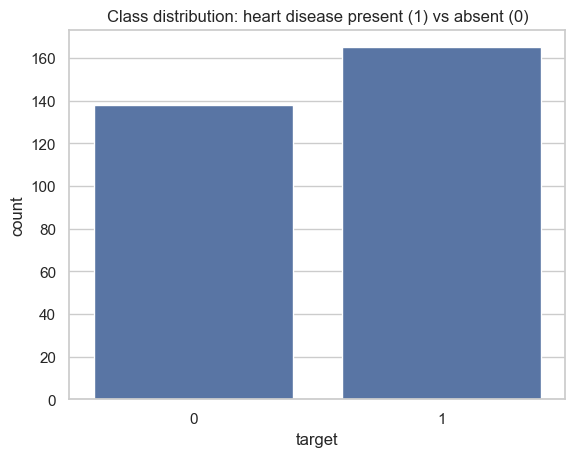
\includegraphics[width=\linewidth]{class_distribution.png}
    \caption{Class distribution (target=1 indicates heart disease).}
  \end{subfigure}
  \hfill
  \begin{subfigure}[t]{0.48\textwidth}
    \centering
    \includegraphics[width=\linewidth]{duplicate_row_counts.png}
    \caption{Duplicate-row count in the raw OpenML frame.}
  \end{subfigure}
  \caption{Dataset profile used for sanity checks.}
\end{figure}

\begin{figure}[t]
  \centering
  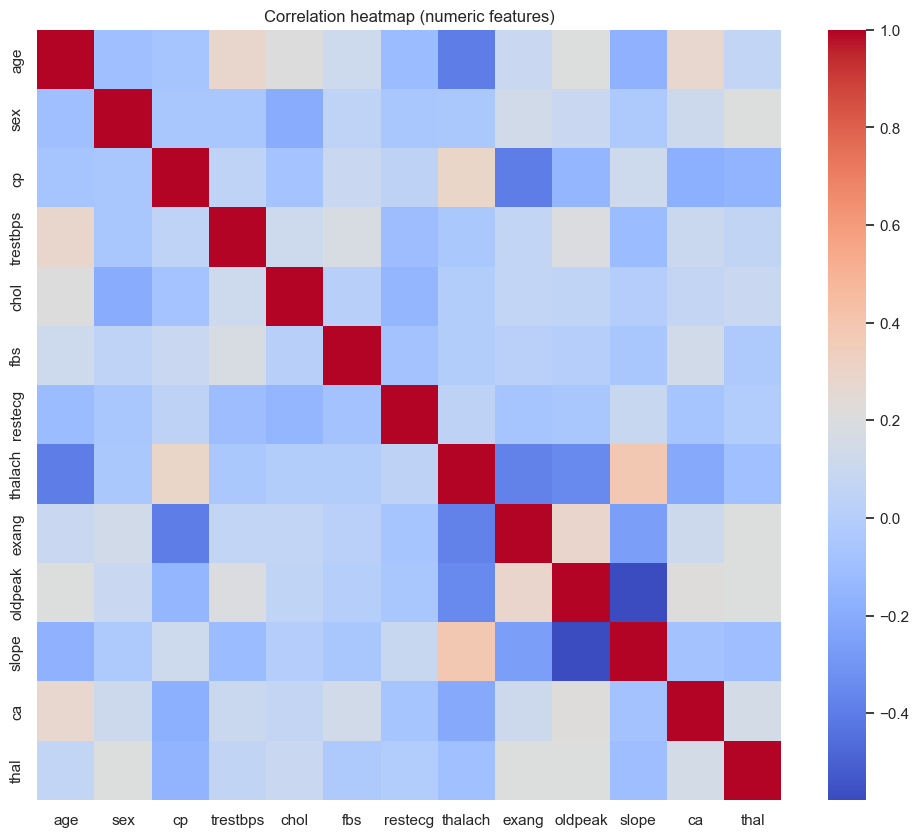
\includegraphics[width=0.62\textwidth]{correlation_heatmap.png}
  \caption{Correlation heatmap of numeric columns.}
\end{figure}

All baseline, deep, custom-grid, ensemble, and fairness scripts are rerun after the heart-disease migration so that outputs are internally consistent. For the custom model, an additional stabilization pass is applied after observing weak early runs: hidden size is reduced, residual depth is reduced, dropout is increased, the maximum learning rate is lowered, and early stopping patience is increased. These changes significantly improve the best custom run compared with earlier unstable configurations.

\subsection{End-to-End Execution Order}
The full execution order is important for reproducibility and consistency. We first regenerate exploratory artifacts and clean split files, then train classical baselines, then deep models, then the 12 custom variants, followed by ensembling and subgroup analysis. Finally, comparison tables and plots are regenerated so that report values are synchronized with the latest outputs. Running this order reduces stale-artifact risk and ensures that each downstream step consumes the correct upstream predictions.

\subsection{Experimental Results and Analysis}
Table 1 summarizes representative leaderboard results from the regenerated comparison outputs. LightGBM provides the best AUC (0.899) and very high recall, with CatBoost close behind at 0.891. Logistic and elastic-net baselines remain highly competitive around 0.857--0.859 AUC, confirming that the dataset contains substantial linear signal after preprocessing. The ensemble reaches 0.878 AUC and improves over many individual models, but does not surpass the best single booster in this split.

\begin{table}[t]
\centering
\small
\caption{Held-out test metrics from regenerated leaderboard.}
\begin{tabular}{lrrrr}
\toprule
Model & ROC-AUC & F1 & Recall & Accuracy \\
\midrule
LightGBM & 0.899 & 0.862 & 1.000 & 0.826 \\
CatBoost & 0.891 & 0.836 & 0.920 & 0.804 \\
Ensemble & 0.878 & 0.711 & 0.640 & 0.717 \\
Elastic Net LR & 0.859 & 0.824 & 0.840 & 0.804 \\
Logistic Regression & 0.857 & 0.824 & 0.840 & 0.804 \\
Random Forest & 0.855 & 0.772 & 0.880 & 0.717 \\
XGBoost & 0.848 & 0.800 & 0.880 & 0.761 \\
HistGradientBoosting & 0.848 & 0.800 & 0.880 & 0.761 \\
Best Custom (balanced) & 0.796 & 0.776 & 0.760 & 0.761 \\
TabTransformerLite & 0.457 & 0.490 & 0.480 & 0.457 \\
\bottomrule
\end{tabular}
\end{table}

\begin{figure}[t]
  \centering
  \includegraphics[width=0.9\textwidth]{model_comparison_auc_top15.png}
  \caption{Top runs ranked by ROC-AUC.}
\end{figure}

\begin{figure}[t]
  \centering
  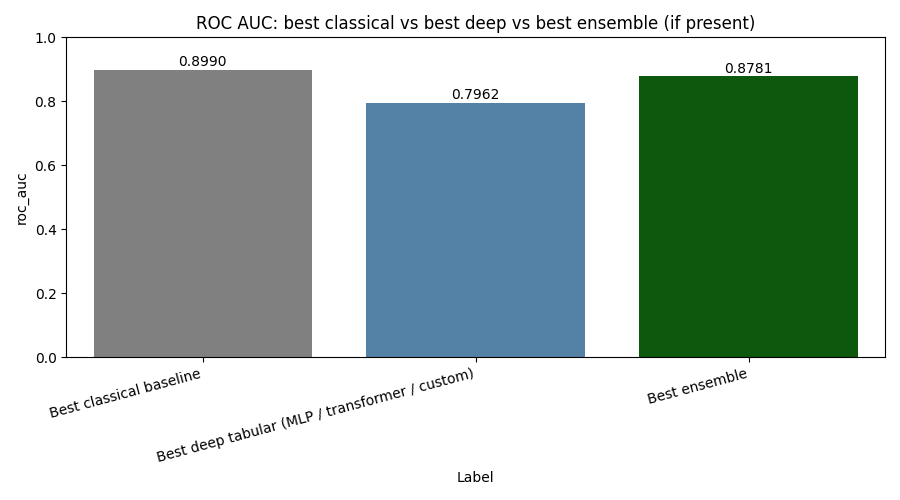
\includegraphics[width=0.85\textwidth]{custom_vs_baseline.png}
  \caption{Comparison of best classical, deep, and ensemble families.}
\end{figure}

Several trends are consistent with expectations for small clinical tabular data. Boosted trees are strongest because they model nonlinear feature interactions efficiently while maintaining favorable bias-variance behavior at this scale. Logistic baselines remain close to top tree models, which suggests meaningful signal is available even through simpler boundaries. Random forest is competitive but generally weaker than boosting, likely because bagging does not refine residual error as aggressively. XGBoost and histogram gradient boosting perform reasonably but slightly below LightGBM and CatBoost on this split, indicating either split sensitivity or hyperparameter fit rather than fundamental weakness.

Deep models show the largest variance. The standard MLP and transformer variants are substantially weaker in this run, and the transformer is the weakest overall by AUC. The most plausible explanation is that one-hot sparse representations and limited sample size make optimization noisy and calibration unstable, while transformer-style token interactions do not have enough data to generalize reliably. The custom residual model improves after stabilization and reaches 0.796 AUC, but still trails the strongest classical models. Within the 12-run custom grid, performance spreads widely, showing that objective design and mitigation weighting can dominate architecture quality in low-data settings.

\subsection{Model-by-Model Interpretation}
The two logistic baselines provide an important anchor for this report. Their strong and stable performance indicates that the dataset contains considerable linear-separable signal after preprocessing. This is valuable because it shows that added complexity must clear a meaningful baseline to be justified. Random forest improves nonlinear expressivity but trails boosted methods, likely because averaging independent trees reduces variance without the same residual-correction strength that boosting provides.

Among boosting methods, LightGBM and CatBoost lead. LightGBM achieves the highest AUC and strong recall, while CatBoost remains close and robust. XGBoost and histogram gradient boosting are still competitive but slightly lower, which may be due to split-specific sensitivity and hyperparameter interaction rather than a structural limitation of those algorithms. The key takeaway is that gradient boosting as a family is consistently reliable for this dataset.

The deep family displays the widest spread. The MLP underperforms likely due to overfitting and unstable probability calibration on a small one-hot feature space. The compact tabular transformer underperforms even more, which is consistent with the idea that attention-based tabular models can be data-hungry and sensitive to architecture scale. The custom residual network shows that deep methods can recover part of the gap after careful stabilization, but outcomes remain highly dependent on objective design and mitigation settings.

\subsection{Deep Learning-Centric Interpretation}
Although the strongest final score is from a tree ensemble, the deep-learning component remains central to the scientific contribution because it exposes where neural tabular modeling breaks under realistic low-data constraints. Rather than treating weaker deep performance as a negative result to hide, we treat it as an evidence-backed finding: architecture capacity alone does not overcome sample scarcity, sparse one-hot inputs, and objective-instability effects.

From a neural-network perspective, three observations are most relevant. First, representation matters: one-hot encoding may be convenient but can be statistically inefficient for small data, suggesting learned categorical embeddings as a higher-priority next step. Second, objective and sampling design matter as much as architecture: the spread across the 12 custom runs shows that mitigation/weighting settings can dominate gradient behavior. Third, calibration matters: several deep runs show acceptable threshold metrics but weak ranking quality, indicating that better probability calibration and validation-driven model selection are necessary for robust deployment behavior.

\subsection{Failure Analysis and Technical Hypotheses}
A recurring pattern in weaker deep runs is disagreement between threshold-dependent metrics and ranking quality. Some models can produce acceptable recall at a selected threshold while still having weak AUC, meaning probability ordering is poor even if one operating point appears usable. This explains why we prioritize ROC-AUC for model-family ranking and use recall/F1 for operating-point interpretation.

For the custom grid, the most likely failure mechanism is weight amplification in a low-sample regime. When class weighting and reweighing interact with limited subgroup-label cells, a small set of examples can disproportionately influence gradients, producing unstable calibration and highly variable subgroup behavior. Another likely contributor is objective mismatch: if checkpoint selection and threshold selection emphasize different criteria, model selection can favor unstable decision boundaries. These hypotheses are consistent with the observed spread across the 12 custom runs.

Subgroup analysis by sex reveals that strong global scores do not imply identical operating behavior. Representative fairness outputs are shown in Table 2. LightGBM preserves high recall in both groups but precision differs, indicating uneven false-positive burden. The ensemble shows more conservative recall in one subgroup. Some custom mitigation combinations produce severe subgroup asymmetry, including near-collapse of recall in one group. These patterns suggest that reweighing can shift errors across groups but does not guarantee uniformly improved subgroup behavior.

\subsection{Fairness Interpretation Limits}
The subgroup results are directionally useful but should not be overinterpreted. With a small dataset, sex-specific supports are limited, so confidence intervals would likely be wide. As a result, subgroup metrics in this report should be read as diagnostics that reveal potential risk patterns, not definitive fairness claims. A stronger fairness study would require repeated resampling, calibration-by-group analysis, and external validation on additional cohorts.

\begin{table}[t]
\centering
\small
\caption{Representative sex-stratified results.}
\begin{tabular}{llrrrr}
\toprule
Model & Sex group & Accuracy & Recall & Precision & ROC-AUC \\
\midrule
LightGBM & 0 & 0.938 & 1.000 & 0.929 & 0.949 \\
LightGBM & 1 & 0.767 & 1.000 & 0.632 & 0.866 \\
Ensemble & 0 & 0.750 & 0.769 & 0.909 & 0.897 \\
Ensemble & 1 & 0.700 & 0.500 & 0.667 & 0.824 \\
Custom (hybrid\_mit\_both) & 0 & 0.688 & 0.692 & 0.900 & 0.872 \\
Custom (hybrid\_mit\_both) & 1 & 0.567 & 0.083 & 0.333 & 0.574 \\
\bottomrule
\end{tabular}
\end{table}

\begin{figure}[t]
  \centering
  \includegraphics[width=\textwidth]{sex_recall_comparison.png}
  \caption{Recall by sex across representative models.}
\end{figure}

\subsection{Statistical Validation Protocol}
Current rankings are based on one stratified split, so close differences should be interpreted cautiously. To strengthen statistical confidence, the next protocol should run 3--5 independent seeds with the same preprocessing and model-search budget, then report mean and standard deviation for ROC-AUC, F1, recall, and accuracy on the held-out test fold. For subgroup analysis, seed-averaged metrics should be supplemented with bootstrap confidence intervals to quantify uncertainty in sex-stratified recall and precision.

This protocol directly addresses two risks in small tabular studies: rank instability among top models and over-interpretation of subgroup gaps from small supports. It also makes the deep-vs-classical comparison more defensible, because performance claims can then be framed as distributions across seeds rather than single-point outcomes.

\subsection{Visual Diagnostics}
The following diagnostics provide rank-oriented evidence (ROC and precision-recall) for one strong classical model (LightGBM) and one neural baseline (MLP). The paired confusion matrices make threshold trade-offs explicit, and the learning-curve diagnostic from gradient boosting training dynamics helps explain why boosting remains stable in this dataset while neural runs are more variable.

\begin{figure}[t]
  \centering
  \begin{subfigure}[t]{0.48\textwidth}
    \centering
    
\includegraphics[width=\linewidth]{roc_curve.png}
    \caption{LightGBM ROC curve.}
  \end{subfigure}
  \hfill
  \begin{subfigure}[t]{0.48\textwidth}
    \centering
    
\includegraphics[width=\linewidth]{pr_curve.png}
    \caption{LightGBM precision-recall curve.}
  \end{subfigure}
  \\
  \begin{subfigure}[t]{0.48\textwidth}
    \centering
    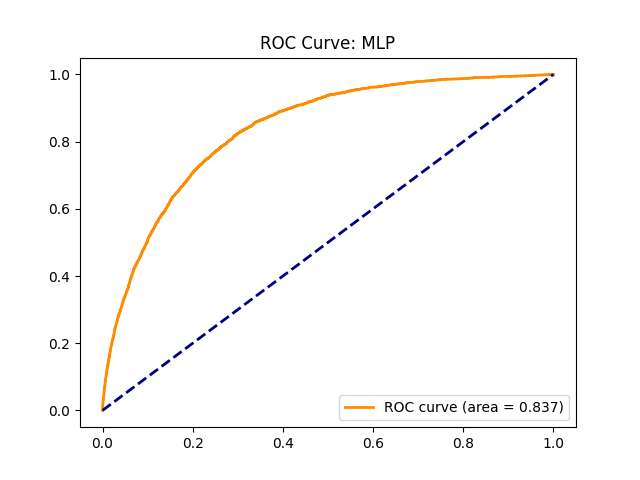
\includegraphics[width=\linewidth]{../outputs/mlp/roc_curve.png}
    \caption{MLP ROC curve.}
  \end{subfigure}
  \hfill
  \begin{subfigure}[t]{0.48\textwidth}
    \centering
    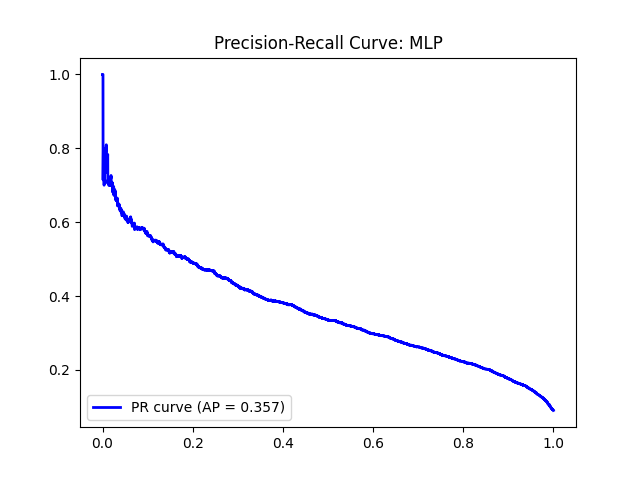
\includegraphics[width=\linewidth]{../outputs/mlp/pr_curve.png}
    \caption{MLP precision-recall curve.}
  \end{subfigure}
  \caption{Representative classical vs neural ranking diagnostics.}
\end{figure}

\begin{figure}[t]
  \centering
  \begin{subfigure}[t]{0.48\textwidth}
    \centering
    
\includegraphics[width=\linewidth]{confusion_matrix.png}
    \caption{LightGBM confusion matrix.}
  \end{subfigure}
  \hfill
  \begin{subfigure}[t]{0.48\textwidth}
    \centering
    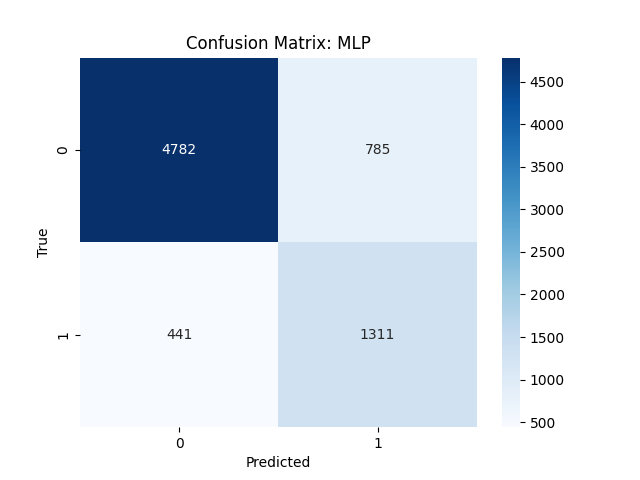
\includegraphics[width=\linewidth]{../outputs/mlp/confusion_matrix.png}
    \caption{MLP confusion matrix.}
  \end{subfigure}
  \caption{Confusion-matrix view of operating-point behavior.}
\end{figure}

\begin{figure}[t]
  \centering
  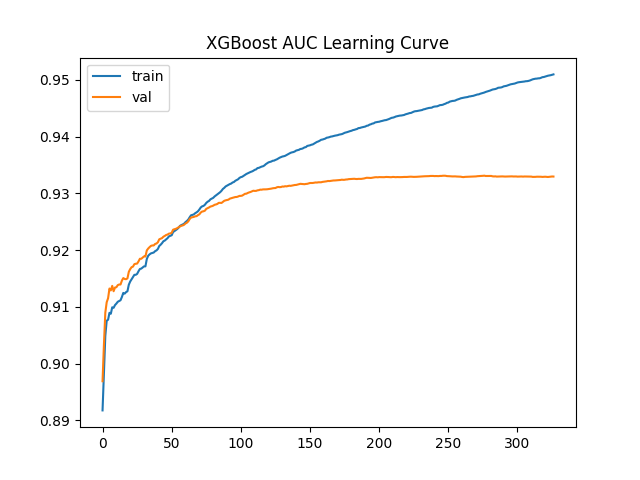
\includegraphics[width=0.72\textwidth]{../outputs/xgboost/learning_curve.png}
  \caption{XGBoost learning-curve diagnostic from training logs.}
\end{figure}

\begin{figure}[t]
  \centering
  \begin{subfigure}[t]{0.48\textwidth}
    \centering
    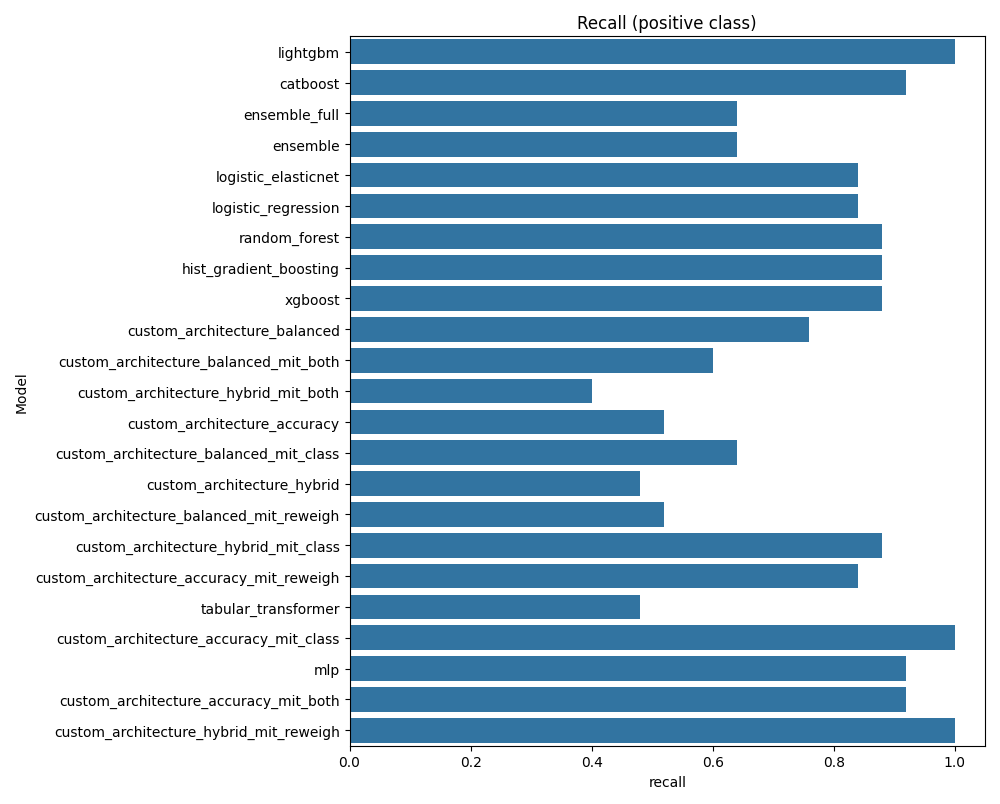
\includegraphics[width=\linewidth]{model_comparison_recall.png}
    \caption{Recall comparison across top models.}
  \end{subfigure}
  \hfill
  \begin{subfigure}[t]{0.48\textwidth}
    \centering
    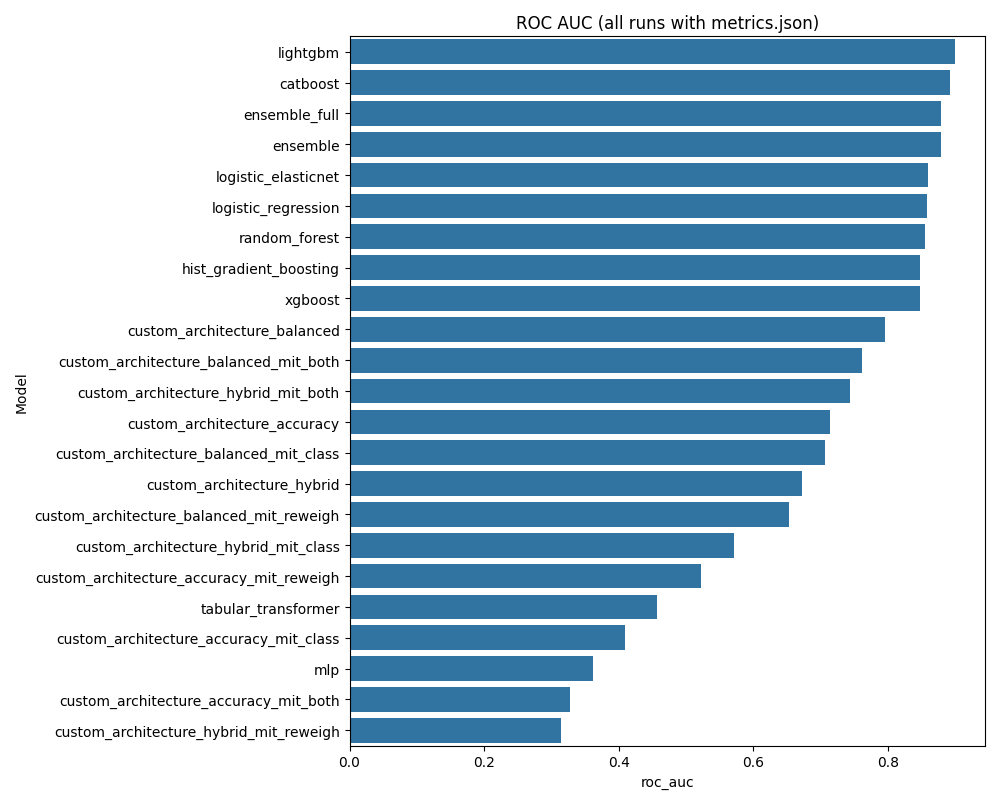
\includegraphics[width=\linewidth]{model_comparison_auc.png}
    \caption{ROC-AUC comparison across top models.}
  \end{subfigure}
  \caption{Global metric comparison diagnostics from regenerated outputs.}
\end{figure}

\begin{figure}[t]
  \centering
  \begin{subfigure}[t]{0.48\textwidth}
    \centering
    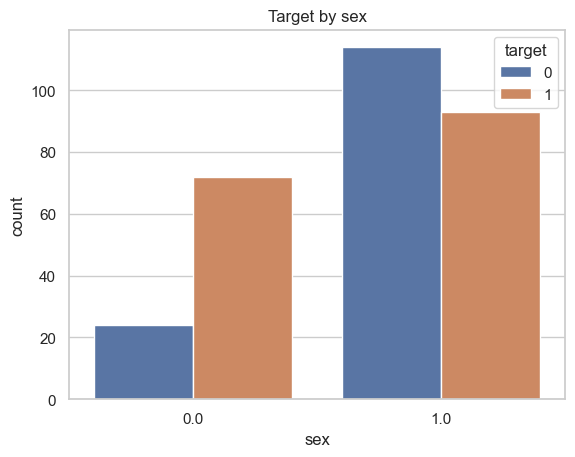
\includegraphics[width=\linewidth]{protected_attribute_distributions.png}
    \caption{Protected-attribute distribution profile.}
  \end{subfigure}
  \hfill
  \begin{subfigure}[t]{0.48\textwidth}
    \centering
    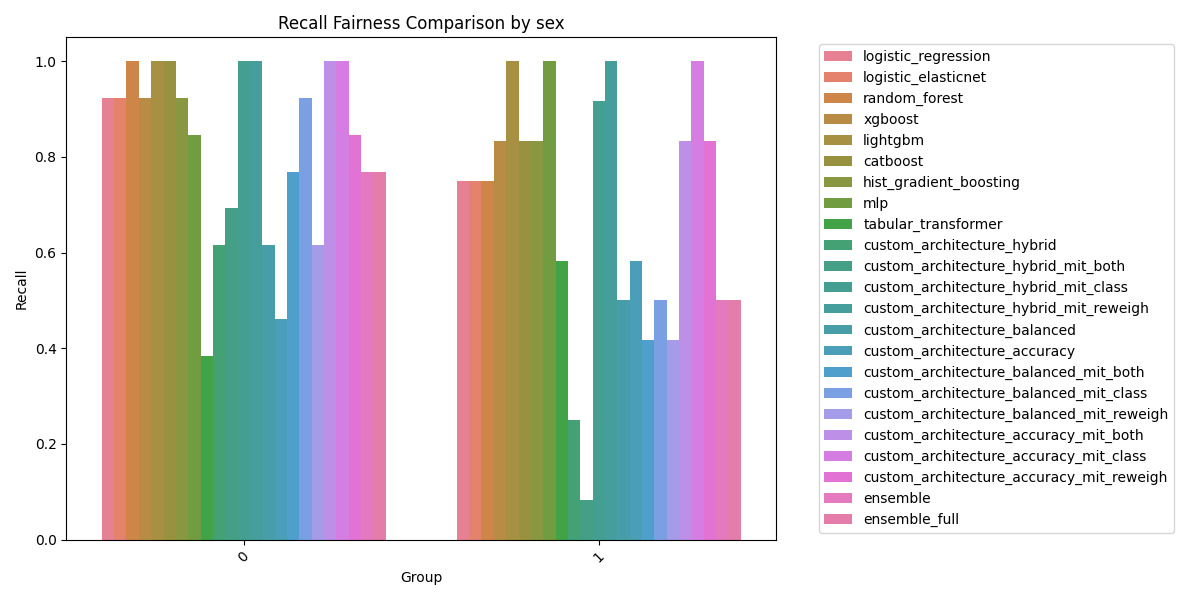
\includegraphics[width=\linewidth]{Sex_recall_comparison.png}
    \caption{Sex-wise recall comparison.}
  \end{subfigure}
  \caption{Fairness-oriented diagnostics used for subgroup interpretation.}
\end{figure}

\begin{figure}[t]
  \centering
  \begin{subfigure}[t]{0.48\textwidth}
    \centering
    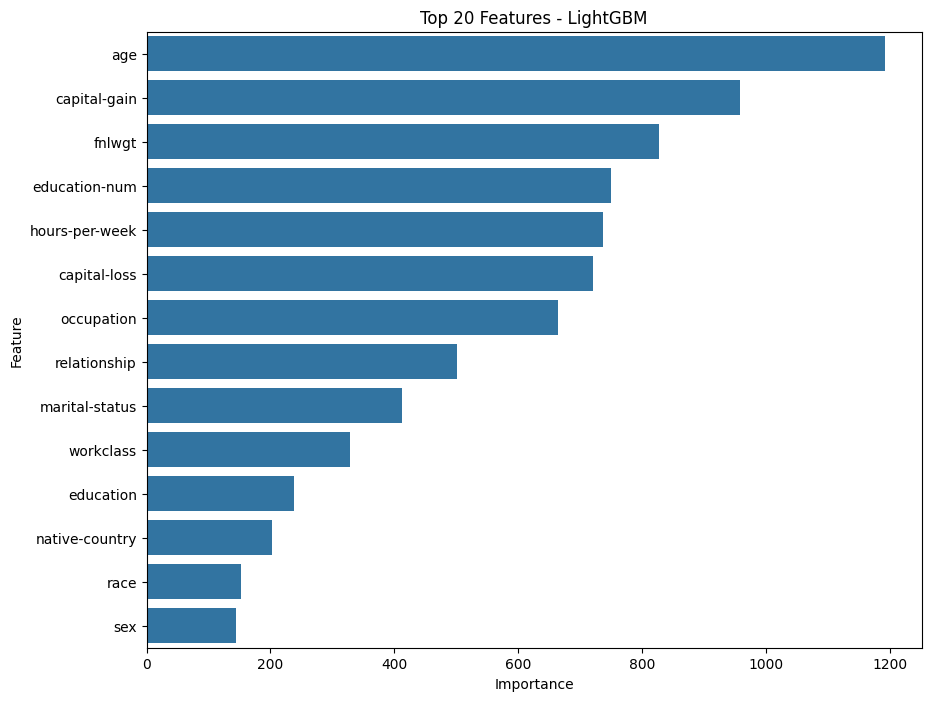
\includegraphics[width=\linewidth]{../outputs/lightgbm/feature_importance.png}
    \caption{LightGBM feature importance.}
  \end{subfigure}
  \hfill
  \begin{subfigure}[t]{0.48\textwidth}
    \centering
    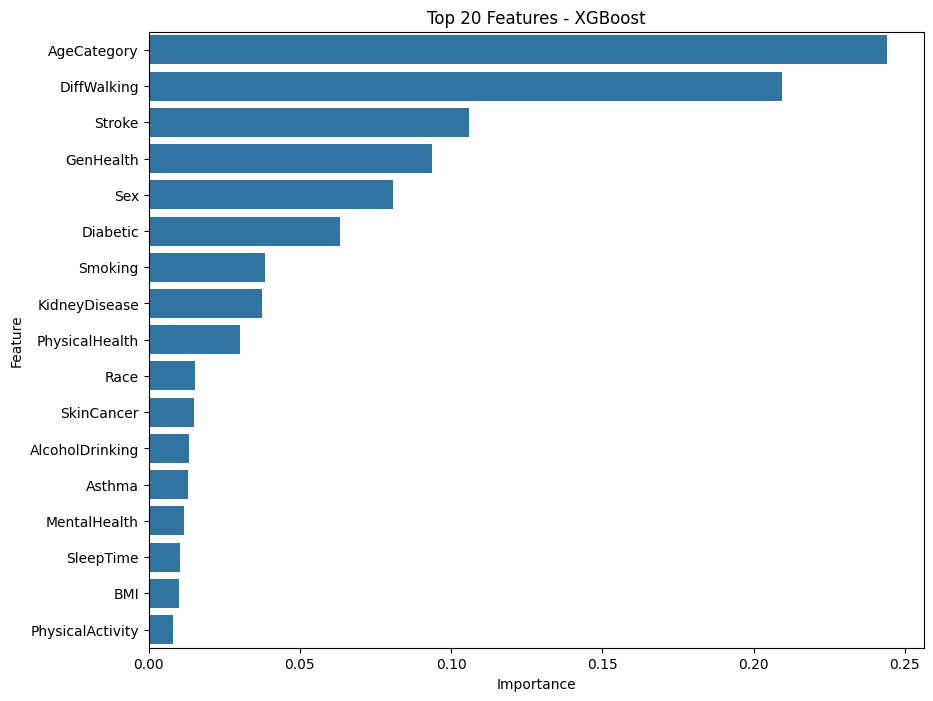
\includegraphics[width=\linewidth]{../outputs/xgboost/feature_importance.png}
    \caption{XGBoost feature importance.}
  \end{subfigure}
  \caption{Tree-model feature attribution diagnostics.}
\end{figure}

\subsection{Natural Next Steps}
The first next step is representation-focused deep learning work: replace one-hot inputs with learned categorical embeddings, then retune regularization and optimizer schedules under fixed data splits. The second is statistical strengthening: execute the multi-seed protocol above and add uncertainty bands to both global and subgroup tables. The third is decision-focused evaluation, where thresholds are selected for specific clinical operating targets and compared using cost-aware criteria instead of single-point summaries. The fourth is external validation on another heart-disease dataset to test whether current rankings hold under distribution shift.

\section{Conclusions}
The main takeaway is that, on this heart-disease benchmark, carefully tuned classical tabular methods remain the most reliable choice. LightGBM and CatBoost lead by AUC, logistic baselines remain unexpectedly strong, and ensembling is useful for robustness but does not automatically beat the best single model. Deep approaches can work in selected configurations, as shown by the improved custom residual run, but they are significantly less stable and more sensitive to objective and mitigation choices in this low-data setting.

The ethical implications are substantial because predictive errors may influence clinical pathways. Fairness analysis in this report shows that global performance can mask subgroup differences in precision and recall, so deployment decisions should not rely on aggregate metrics alone. Transparency about training data limitations, subgroup behavior, threshold trade-offs, and failure modes is therefore essential. Any real clinical use would require prospective validation on broader populations, rigorous governance, and a clear human-in-the-loop accountability framework where models support clinicians rather than replace them.

\begin{thebibliography}{99}
\bibitem{detrano1989}
R. Detrano et al., ``International application of a new probability algorithm for the diagnosis of coronary artery disease,'' \emph{The American Journal of Cardiology}, 64(5), 1989.

\bibitem{uci_heart}
J. Janosi, W. Steinbrunn, M. Pfisterer, and R. Detrano, ``Heart Disease Data Set,'' UCI Machine Learning Repository, 1988.

\bibitem{openml}
J. Vanschoren et al., ``OpenML: networked science in machine learning,'' \emph{SIGKDD Explorations}, 15(2), 2014.

\bibitem{chen2016xgboost}
T. Chen and C. Guestrin, ``XGBoost: A Scalable Tree Boosting System,'' in \emph{Proceedings of KDD}, 2016.

\bibitem{ke2017lightgbm}
G. Ke et al., ``LightGBM: A Highly Efficient Gradient Boosting Decision Tree,'' in \emph{NeurIPS}, 2017.

\bibitem{prokhorenkova2018catboost}
L. Prokhorenkova et al., ``CatBoost: Unbiased Boosting with Categorical Features,'' in \emph{NeurIPS}, 2018.

\bibitem{gorishniy2021revisiting}
Y. Gorishniy, I. Rubachev, V. Khrulkov, and A. Babenko, ``Revisiting Deep Learning Models for Tabular Data,'' in \emph{NeurIPS}, 2021.

\bibitem{kamiran2012data}
F. Kamiran and T. Calders, ``Data Preprocessing Techniques for Classification without Discrimination,'' \emph{Knowledge and Information Systems}, 33(1), 2012.

\bibitem{barocas2023fairness}
S. Barocas, M. Hardt, and A. Narayanan, \emph{Fairness and Machine Learning: Limitations and Opportunities}, MIT Press, 2023. \url{https://fairmlbook.org}
\end{thebibliography}

\end{document}